\chapter{Tools and Technologies}

\justify
{\myprojectname} encompasses a wide range of tools and technologies that facilitate the creation, deployment, and maintenance of applications. From integrated development environments (IDEs) for coding to version control systems (VCS) for collaboration, programming languages, frameworks, database management systems (DBMS), containerization tools, continuous integration/continuous deployment (CI/CD) pipelines, cloud platforms, testing tools, API development tools, code editors, project management platforms, security tools, and monitoring/logging solutions, the software development landscape is rich and diverse, catering to various aspects of the development lifecycle.
\section{Tools}
\justify

React Native is a popular open-source framework developed by Facebook for building mobile applications using JavaScript and React. It allows developers to create native mobile apps for both iOS and Android platforms using a single codebase. However, since you specifically asked about Android apps, I'll focus on that aspect.

% \begin{figure}
%   \centering
%   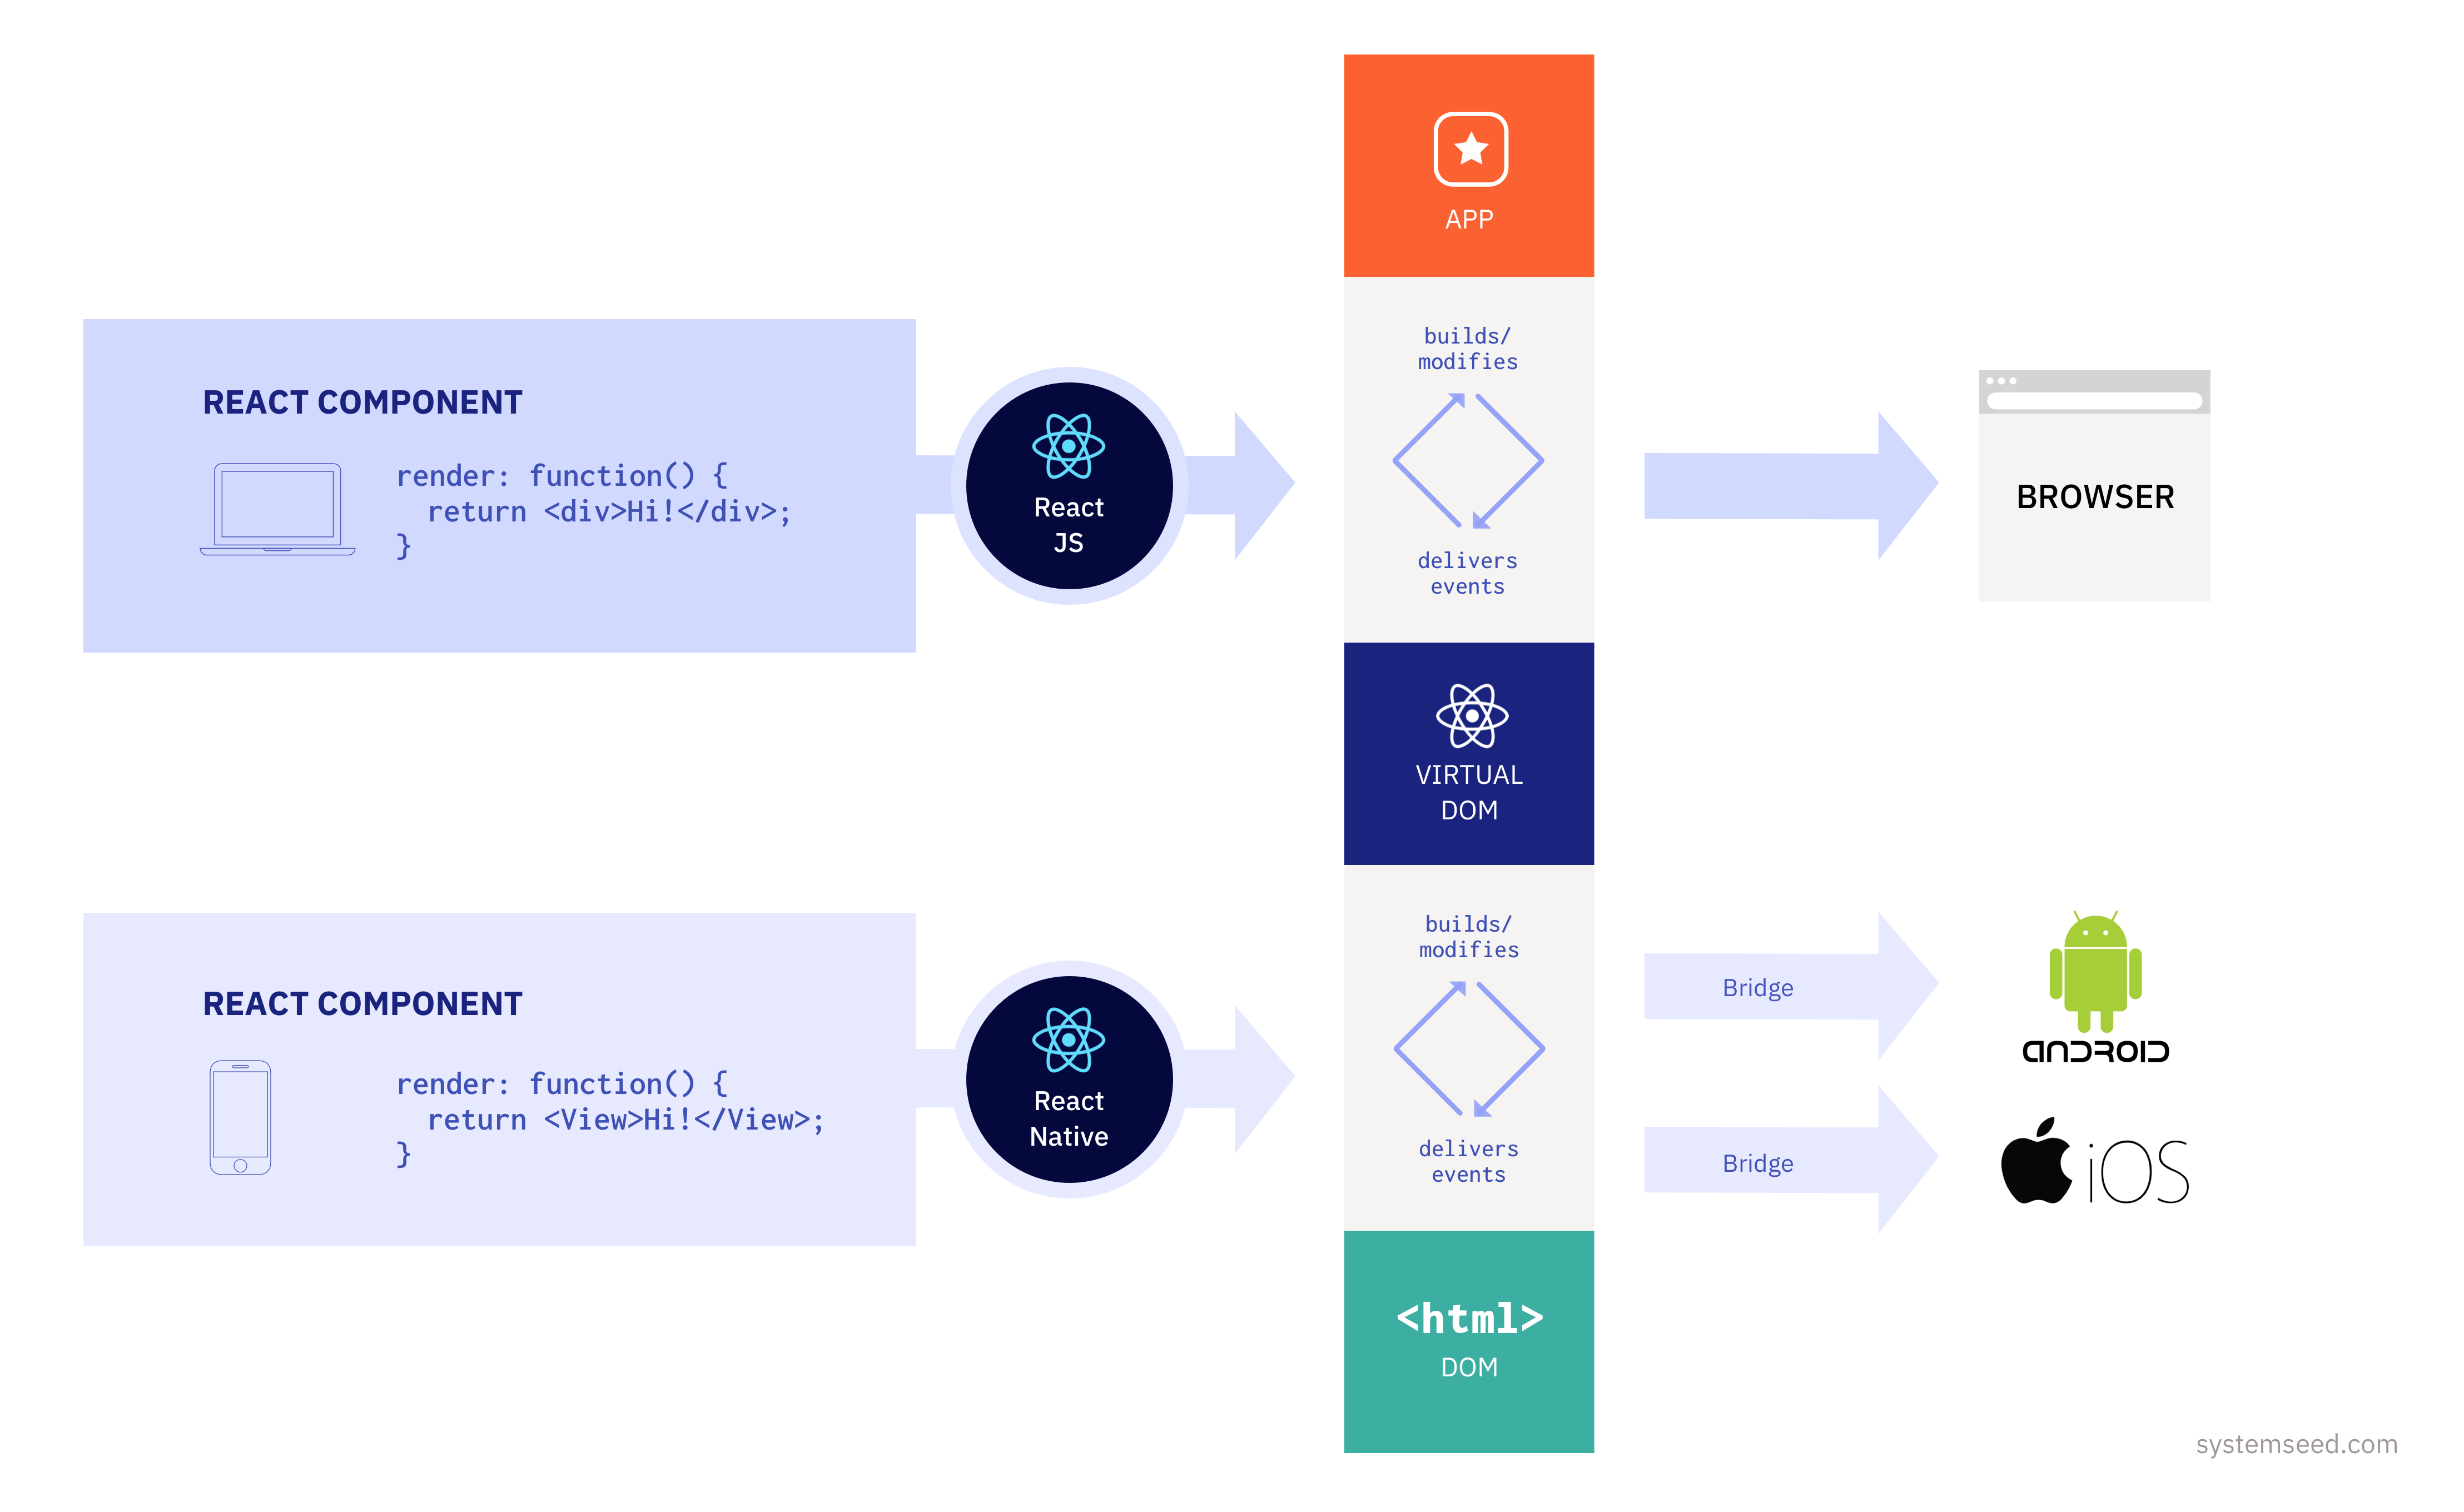
\includegraphics[width=0.90\linewidth]{Media/react-diagram_3.png}
%   \caption{React Native}
%   \label{fig:React Native}
% \end{figure}

\begin{enumerate}
  \item \textbf{Visual Studio Code}: Used Visual Studio Code to design the OSINT Software and also used 
  
  \item \textbf{Flipper}: One of the primary advantages of React Native is its ability to support cross-platform development. Developers can write code once and deploy it on both iOS and Android platforms, saving time and effort compared to building separate native apps for each platform.
  
  \item \textbf{React Native Debugger}: React Native allows developers to create native components using JavaScript, which are then rendered using native APIs. This approach enables the development of high-performance apps with a native look and feel, as the components are rendered using the underlying platform's UI elements.
  
  \item \textbf{HTTPie}: React Native includes a feature called hot reloading, which allows developers to see the changes they make to the code in real-time without restarting the app. This can significantly speed up the development process and improve productivity.
  
  \item \textbf{Android Studio}: React Native provides access to native modules and APIs through a bridge mechanism. This means developers can integrate platform-specific functionalities such as camera, geolocation, push notifications, etc., into their apps seamlessly.
  
  \item \textbf{Android Emulator}: React Native has a vibrant ecosystem of third-party libraries, plugins, and community-contributed components that developers can leverage to add additional features and functionalities to their apps.
  
  \item \textbf{Git}: While React Native offers good performance out of the box, developers can further optimize their apps for performance by implementing best practices, using efficient code patterns, and utilizing tools like performance profiling and debugging tools provided by React Native.
  
  \item \textbf{Chromium Browser}: React Native supports various testing and debugging tools, including Jest for unit testing, React Native Debugger for debugging, and tools like Flipper for inspecting app performance and behavior. 

  \item \textbf{DBeaver}: React Native supports various testing and debugging tools, including Jest for unit testing, React Native Debugger for debugging, and tools like Flipper for inspecting app performance and behavior. 

  \item \textbf{Nginx}: React Native supports various testing and debugging tools, including Jest for unit testing, React Native Debugger for debugging, and tools like Flipper for inspecting app performance and behavior. 

  \item \textbf{Puppeteer}: React Native supports various testing and debugging tools, including Jest for unit testing, React Native Debugger for debugging, and tools like Flipper for inspecting app performance and behavior. 
  
  \begin{figure}
    \centering
    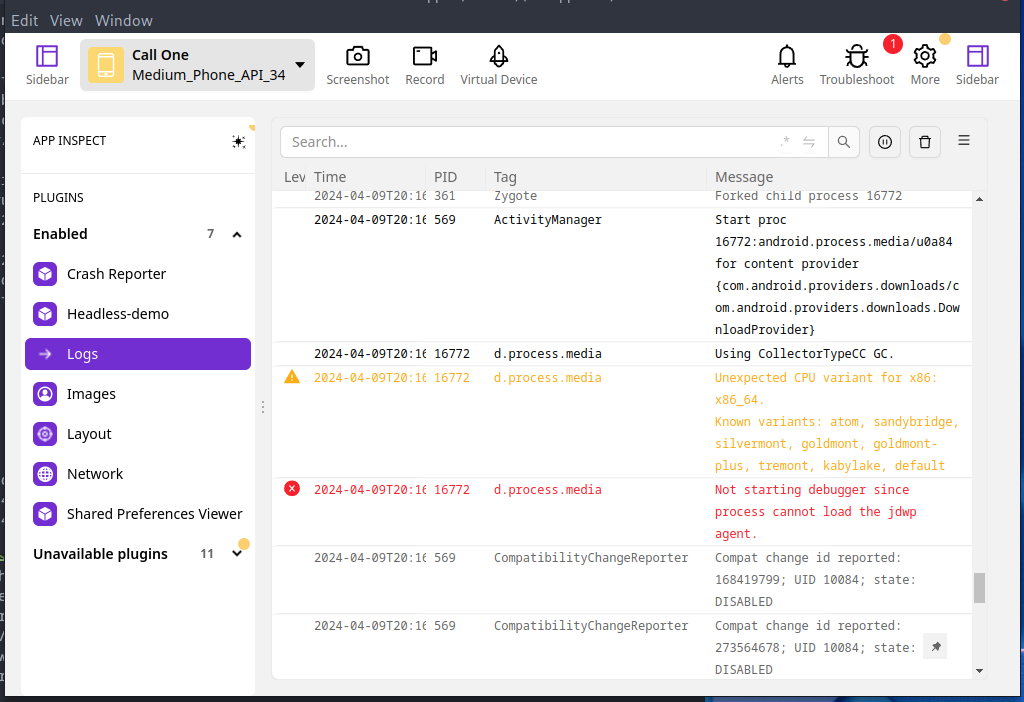
\includegraphics[width=1\linewidth]{Media//Chapter 6/flipper.png}
    \caption{Flipper Debugging}
    \label{fig:Flipper Debugging}
  \end{figure}
\end{enumerate}


\section{Technologies}
\justify

React Native is a popular open-source framework developed by Facebook for building mobile applications using JavaScript and React. It allows developers to create native mobile apps for both iOS and Android platforms using a single codebase. However, since you specifically asked about Android apps, I'll focus on that aspect.

% \begin{figure}
%   \centering
%   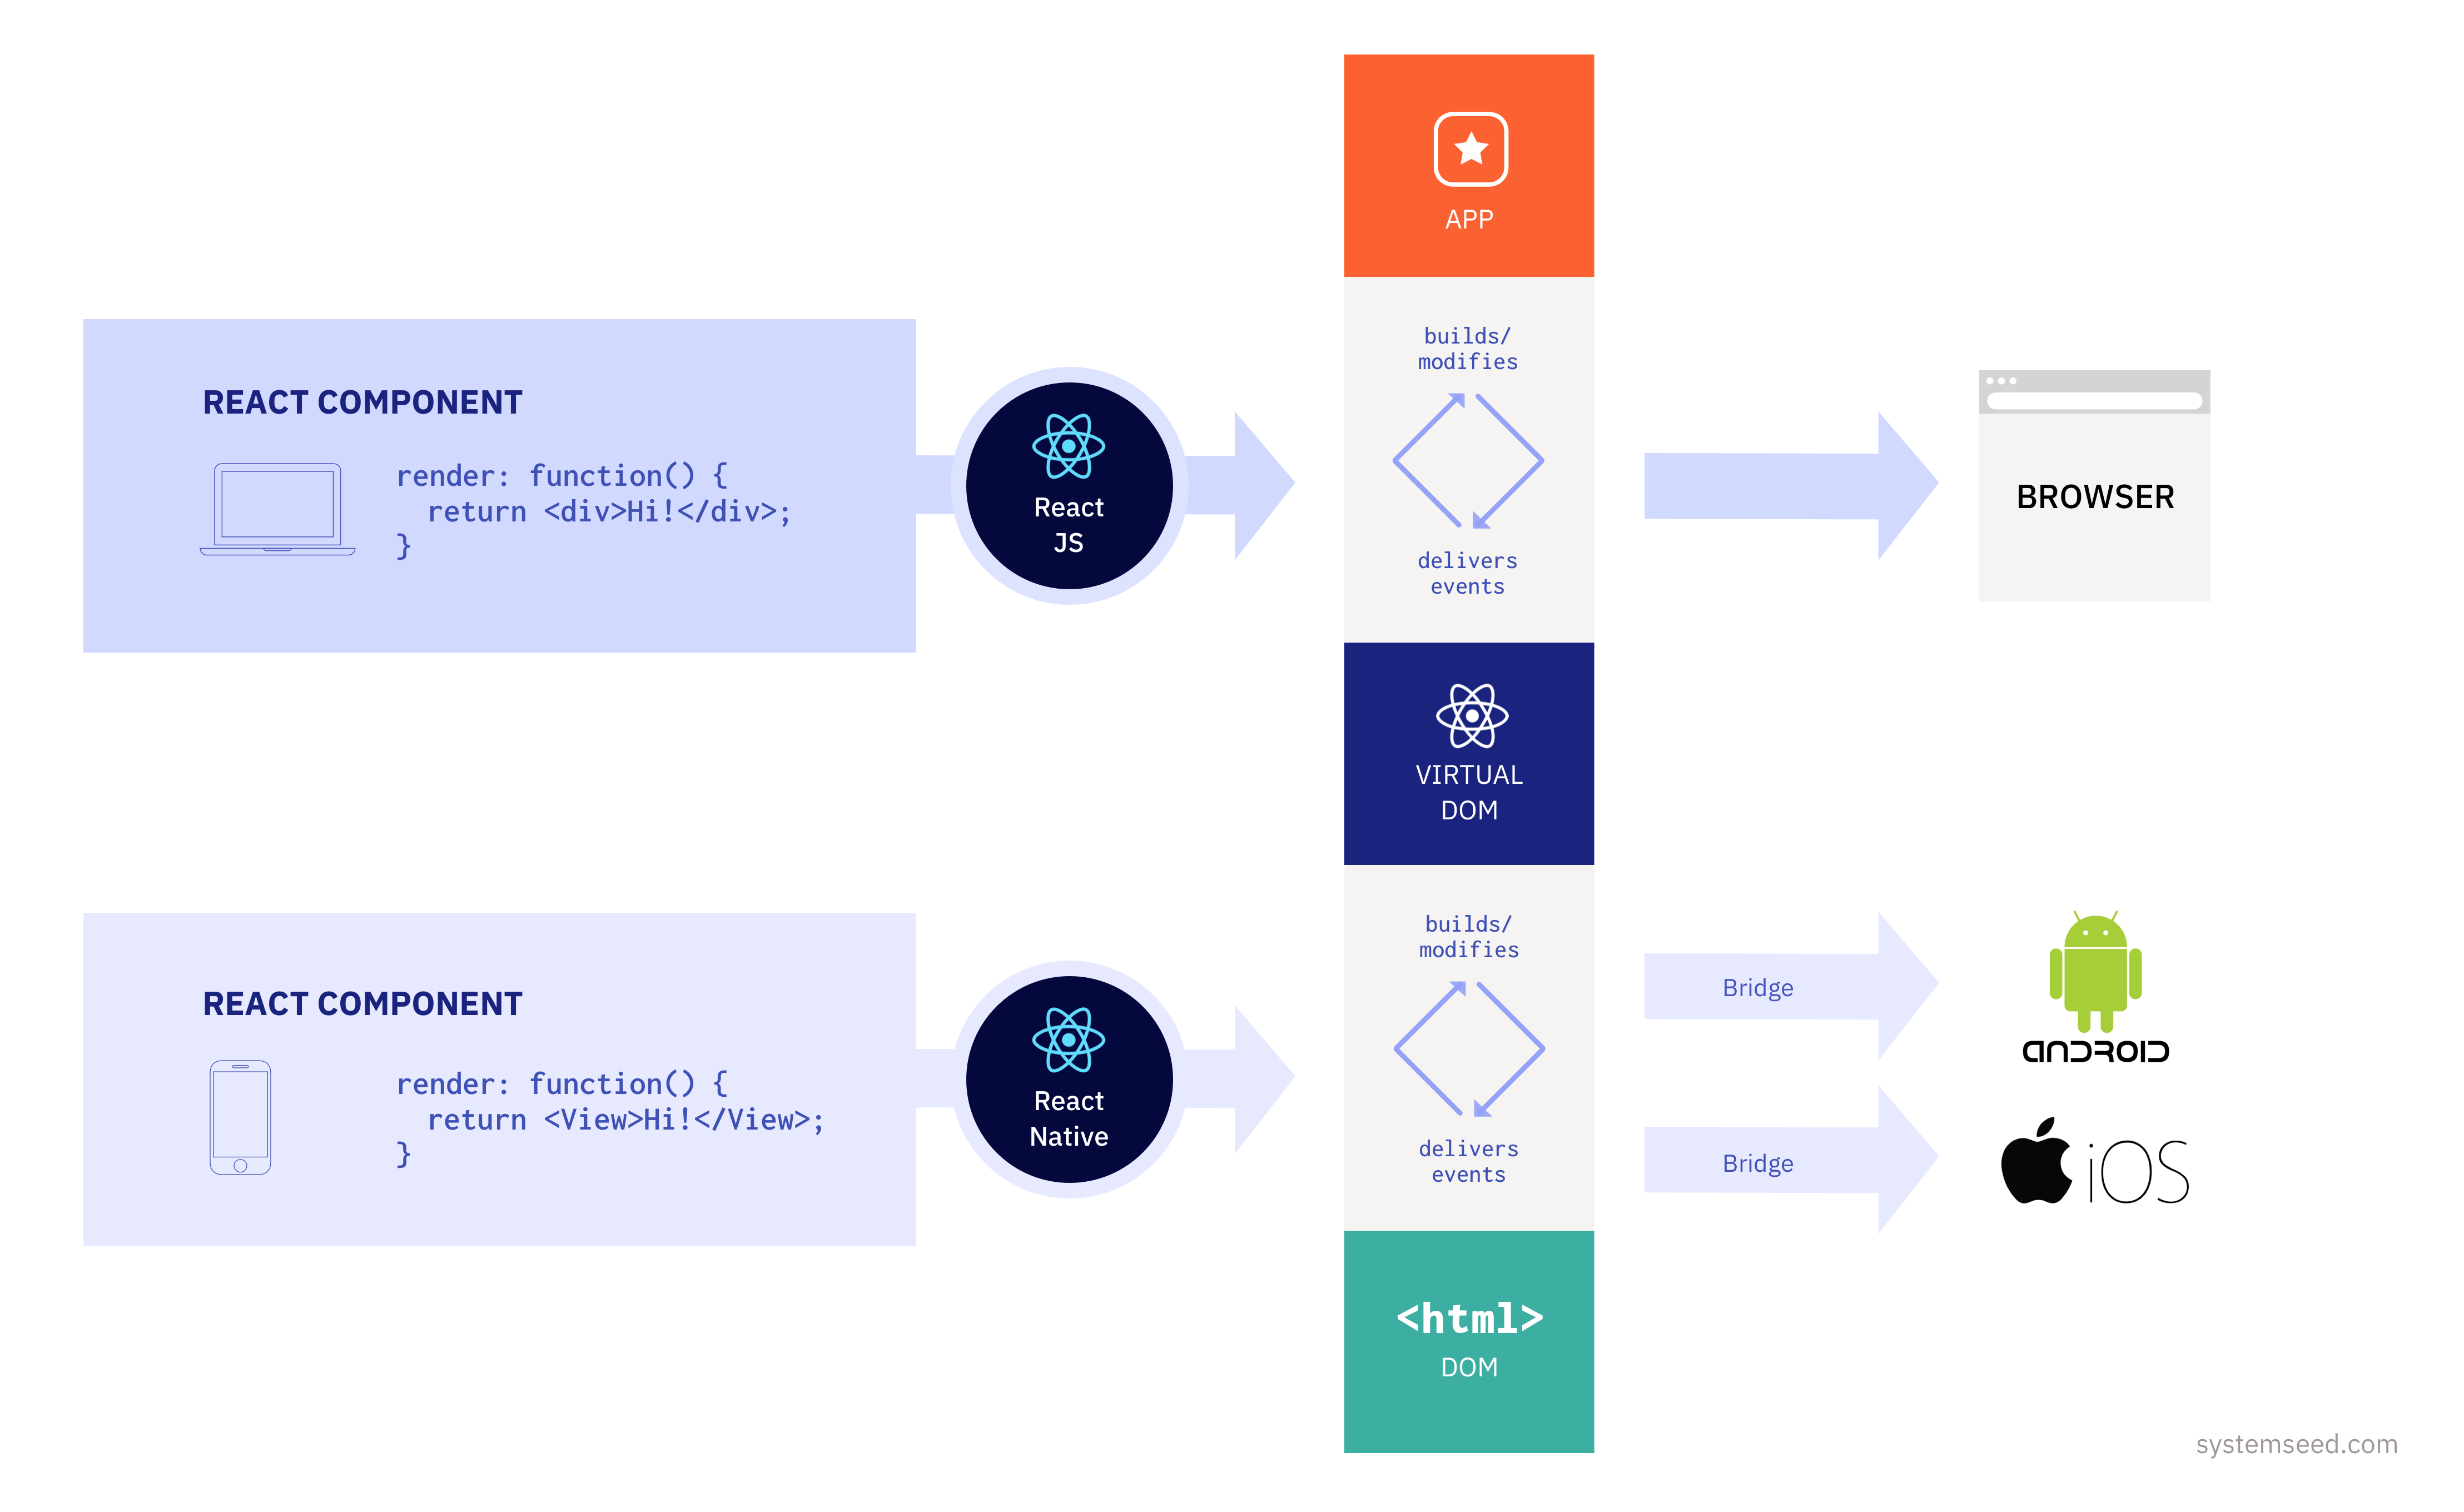
\includegraphics[width=0.90\linewidth]{Media/react-diagram_3.png}
%   \caption{React Native}
%   \label{fig:React Native}
% \end{figure}

\begin{enumerate}
  \item \textbf{React Native}: React Native utilizes JavaScript as the programming language and React as the JavaScript library for building user interfaces. This combination enables developers to write code in a familiar language and leverage React's component-based architecture for UI development.
  
  \item \textbf{Kotlin}: One of the primary advantages of React Native is its ability to support cross-platform development. Developers can write code once and deploy it on both iOS and Android platforms, saving time and effort compared to building separate native apps for each platform.
  
  \item \textbf{JavaScript}: React Native allows developers to create native components using JavaScript, which are then rendered using native APIs. This approach enables the development of high-performance apps with a native look and feel, as the components are rendered using the underlying platform's UI elements.
  
  \item \textbf{TypeScript}: React Native includes a feature called hot reloading, which allows developers to see the changes they make to the code in real-time without restarting the app. This can significantly speed up the development process and improve productivity.
  
  \item \textbf{Express.js}: React Native provides access to native modules and APIs through a bridge mechanism. This means developers can integrate platform-specific functionalities such as camera, geolocation, push notifications, etc., into their apps seamlessly.
  
  \item \textbf{Node.js}: React Native has a vibrant ecosystem of third-party libraries, plugins, and community-contributed components that developers can leverage to add additional features and functionalities to their apps.
  
  \item \textbf{Crypto-js}: While React Native offers good performance out of the box, developers can further optimize their apps for performance by implementing best practices, using efficient code patterns, and utilizing tools like performance profiling and debugging tools provided by React Native.

  \item \textbf{PostgreSQL}: While React Native offers good performance out of the box, developers can further optimize their apps for performance by implementing best practices, using efficient code patterns, and utilizing tools like performance profiling and debugging tools provided by React Native.
 
  \item \textbf{React Native Firebase}: React Native supports various testing and debugging tools, including Jest for unit testing, React Native Debugger for debugging, and tools like Flipper for inspecting app performance and behavior. 
  
  \item \textbf{JSON Web Tokens (JWT)}: While React Native offers good performance out of the box, developers can further optimize their apps for performance by implementing best practices, using efficient code patterns, and utilizing tools like performance profiling and debugging tools provided by React Native.
  
  \item \textbf{PDFKit}: While React Native offers good performance out of the box, developers can further optimize their apps for performance by implementing best practices, using efficient code patterns, and utilizing tools like performance profiling and debugging tools provided by React Native.
  
  \item \textbf{Baileys (WhatsApp Client)}: While React Native offers good performance out of the box, developers can further optimize their apps for performance by implementing best practices, using efficient code patterns, and utilizing tools like performance profiling and debugging tools provided by React Native.
  

  \begin{figure}
    \centering
    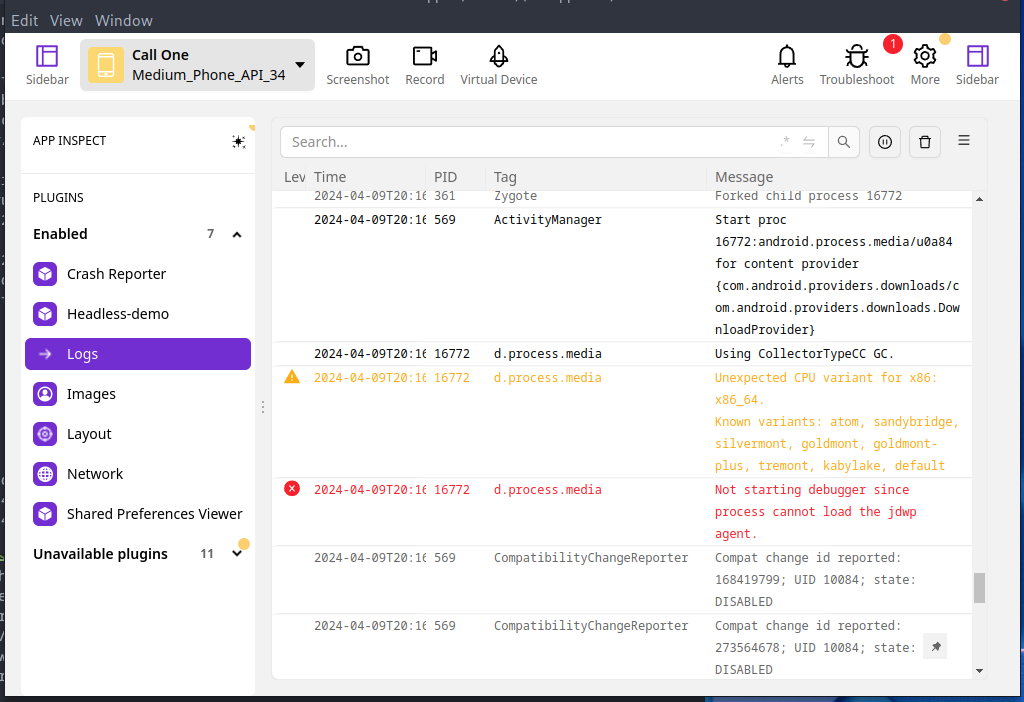
\includegraphics[width=1\linewidth]{Media//Chapter 6/flipper.png}
    \caption{Flipper Debugging}
    \label{fig:Flipper Debugging Tool}
  \end{figure}
\end{enumerate}


\section{Kotlin}

In our Android application development, Kotlin played a crucial role in implementing various functionalities to enhance user experience and ensure data security. This section discusses how Kotlin was used for phone call modules, phone state receiver, and AES encryption for transmitting data to the backend.

\subsection{Phone Call Modules}

Kotlin was utilized to create phone call modules within our app, allowing users to make phone calls directly from the application. This feature streamlined the communication process and provided a seamless experience for users. Key aspects of the phone call modules include:

\begin{enumerate}
  \item Initiating outgoing calls from within the app.
  \item Integrating call management functionalities, such as call duration tracking and call logs.
  \item Ensuring compatibility with different Android devices and versions.
\end{enumerate}

Kotlin's concise syntax and robust features enabled us to develop efficient phone call modules that integrated seamlessly with the app's user interface and functionality.

\subsection{Phone State Receiver}

A phone state receiver implemented in Kotlin was used to detect various call events, including incoming calls, outgoing calls, and ongoing calls. This receiver played a crucial role in managing call-related actions within the app. Key functionalities of the phone state receiver include:

\begin{enumerate}
  \item Detecting incoming calls and displaying caller information.
  \item Monitoring call status changes, such as call answered, call ended, etc.
  \item Handling call-related actions, such as rejecting incoming calls or pausing ongoing calls.
\end{enumerate}

Kotlin's event handling capabilities and compatibility with Android's telephony APIs made it a suitable choice for implementing the phone state receiver.

\subsection{AES Encryption for Data Transmission}

To ensure data security during data transmission to the backend server, AES (Advanced Encryption Standard) encryption was implemented using Kotlin. This encryption technique was applied to encrypt user data and queries before transmitting them over the network. Key aspects of AES encryption integration include:

\begin{enumerate}
  \item Encrypting sensitive user information, such as credentials and personal data, to protect against unauthorized access.
  \item Encrypting data queries to maintain confidentiality and integrity during transmission.
  \item Implementing secure key management practices to generate and store encryption keys securely.
\end{enumerate}


\section{PostgreSQL}

In our application's backend infrastructure, we leveraged PostgreSQL as the database management system for storing user information securely and efficiently. This section outlines how PostgreSQL was utilized to store user data, including the storage of JSON objects in an array format and optimizing queries for fast retrieval.

We designed a PostgreSQL database schema to accommodate various types of user information, such as user profiles, preferences, transactions, and more. The database tables were structured to efficiently store and manage user data while ensuring data integrity and scalability.

For storing JSON objects, we utilized PostgreSQL's native support for JSON data types. Specifically, we stored JSON objects in arrays within PostgreSQL tables, allowing us to organize and manage structured data effectively.


\begin{enumerate}
  \item \textbf{Structured Data Storage}: JSON arrays provided a structured format for storing related data elements, such as an array of user preferences or a list of user transactions.
  
  \item \textbf{Flexible Data Retrieval}: PostgreSQL's JSON functions and operators allowed us to query and manipulate JSON data within arrays, facilitating flexible data retrieval and processing.
  
  \item \textbf{Reduced Data Redundancy}: Storing JSON objects in arrays minimized data redundancy by grouping related data elements together, optimizing storage space and database performance.
  
  \item \textbf{Indexing}: We created appropriate indexes on database columns used in frequent queries, such as user IDs, to accelerate data retrieval operations.
  
  \item \textbf{Query Optimization}: We optimized SQL queries by utilizing PostgreSQL's query planner and execution engine, ensuring optimal query performance and resource utilization.
  
  \item \textbf{Caching}: Where applicable, we implemented caching mechanisms at the application layer to reduce database load and improve response times for frequently accessed data.
\end{enumerate}

To ensure fast and efficient retrieval of user information from the PostgreSQL database, we optimized database queries using various techniques, including:


By combining efficient database schema design, storage of JSON objects in arrays, and query optimization techniques, we achieved fast and reliable data retrieval capabilities from the PostgreSQL database, enhancing overall application performance and user experience.



\section{React Native Firebase}

In our mobile application development using React Native, we leveraged React Native Firebase for implementing Google SignIn functionality. This section outlines how React Native Firebase facilitated seamless integration with Google SignIn and enhanced user authentication capabilities.

\subsection{Integration with React Native Firebase}

React Native Firebase provides a comprehensive set of Firebase services for React Native apps, including authentication services like Google SignIn. By integrating React Native Firebase into our project, we gained access to Firebase's authentication APIs, simplifying the implementation of Google SignIn.

\section{Flipper}

Flipper is a powerful debugging and development tool created by Facebook for mobile app developers. It provides a suite of features and capabilities that streamline the debugging and testing process, enhancing productivity and improving the overall quality of mobile applications.

\subsection{Key Features of Flipper}

\begin{enumerate}
  \item \textbf{UI Inspector}: Flipper allows developers to inspect and debug the user interface (UI) of their mobile apps in real-time. Developers can view the layout hierarchy, inspect UI elements, and identify issues or inconsistencies easily.
  
  \item \textbf{Network Inspector}: With Flipper's network inspector, developers can monitor network requests made by their app, view request and response details, analyze network performance, and debug network-related issues efficiently.
  
  \item \textbf{Database Viewer}: Flipper provides a database viewer tool that allows developers to inspect and interact with local databases used by their mobile apps. This feature is particularly useful for debugging data storage and retrieval functionalities.
  
  \item \textbf{Performance Profiling}: Flipper offers performance profiling tools that enable developers to analyze app performance metrics, identify performance bottlenecks, and optimize app performance for better user experience.
  
  \item \textbf{Crash Reporting}: Flipper integrates with crash reporting services, providing developers with insights into app crashes, error logs, and crash analytics. This helps in identifying and resolving critical issues that impact app stability.
\end{enumerate}


\section{JSON Web Tokens (JWT)}

JSON Web Tokens (JWT) are a popular method for managing sessions and authentication in web and mobile applications, including Android apps. In our Android app development, we leveraged JWT for secure and efficient session management. This section outlines how JWT tokens were utilized to manage user sessions in our Android app.

\subsection{JWT Token Generation}

When a user successfully logs in or authenticates in our Android app, a JWT token is generated by the backend server. This JWT token contains encoded user information, such as user ID, roles, and expiration time. The JWT token is then securely stored on the client-side, typically in the app's local storage or shared preferences.

\subsection{Token-Based Authentication}

For subsequent API requests or operations requiring authentication, the JWT token is sent along with the request headers. The backend server verifies the JWT token's authenticity and validity before processing the request. This token-based authentication mechanism eliminates the need for storing session information on the server-side, reducing server load and improving scalability.

\subsection{Token Expiration and Refresh}

JWT tokens have an expiration time set during token generation. When a JWT token expires, the client app can request a new token using a refresh token mechanism. The refresh token is a separate token with a longer expiration time, used to obtain a new JWT token without requiring the user to log in again. This ensures seamless and continuous session management in the app.


\section{Express.js}
In our application's backend development, we utilized Express.js, a popular Node.js framework, to build robust and scalable APIs for handling various functionalities. This section delves into how Express.js was used along with TypeScript for creating APIs, integrating with Next.js, and implementing encryption for secure data handling.

\subsection{APIs for User Contacts and Call Logs}

Using Express.js, we created RESTful APIs to manage user contacts and call logs. These APIs allowed users to:

\begin{enumerate}
  \item Store and retrieve user contacts, including name, phone number, and additional details.
  \item Log incoming and outgoing calls, along with call duration, timestamps, and caller/callee information.
  \item Perform CRUD operations on contacts and call logs, enabling efficient data management.
\end{enumerate}

Express.js's middleware and routing capabilities facilitated the implementation of these APIs, providing a structured and organized approach to backend development.

\subsection{AES Encryption for Secure Query Handling}

To enhance data security, we implemented AES (Advanced Encryption Standard) encryption for handling encrypted queries, especially when searching for a phone number. Key aspects of AES encryption integration include:

\begin{enumerate}
  \item Encrypting user queries containing sensitive information, such as phone numbers, before processing them in the backend.
  \item Decryption of encrypted queries using the AES decryption algorithm to retrieve relevant data securely.
  \item Utilizing secure key management practices to generate and manage encryption keys for AES encryption and decryption.
\end{enumerate}

By incorporating AES encryption, we ensured that user data and queries remained secure and protected against unauthorized access or interception.

\subsection{Integration with Next.js as a Custom Server}

Express.js was integrated as a custom server with Next.js, a React framework for frontend development, to run both backend and frontend on the same server. This integration provided several benefits:

\begin{enumerate}
  \item Simplified deployment and hosting, with a single server instance serving both backend APIs and frontend UI components.
  \item Improved performance and reduced latency due to server-side rendering (SSR) capabilities of Next.js.
  \item Seamless communication between backend APIs and frontend components, enhancing user experience and application responsiveness.
\end{enumerate}

Express.js and Next.js integration offered a cohesive development environment, streamlining the development and deployment process of our application.

\subsection{TypeScript}

For enhanced code quality and maintainability, we leveraged TypeScript with Express.js. TypeScript provided:

\begin{enumerate}
  \item Static typing and type checking, preventing type-related errors and improving code reliability.
  \item Better code documentation and readability with explicit type definitions for variables, functions, and API contracts.
  \item Improved development experience with features like code completion, refactoring tools, and type inference.
\end{enumerate}

TypeScript's integration with Express.js facilitated a more robust and structured backend codebase, enhancing code quality and developer productivity.


\section{Puppeteer}

In our software, we employed Puppeteer, a Node.js library, to scrape images associated with a phone number from Google Contacts. This section details how Puppeteer was used for this purpose and the steps involved in the scraping process. we installed Puppeteer as a Node.js dependency in our project using npm or yarn. Puppeteer provides a high-level API for controlling headless Chrome or Chromium browsers, making it suitable for automating web scraping tasks.


\section{PDFKit}

In our information gathering and analysis process, we utilized PDFKit, a Node.js library, to create a comprehensive OSINT (Open-Source Intelligence) report. This note outlines how PDFKit was employed to generate professional and structured reports based on gathered intelligence.

% \begin{figure}
%     \centering
%     
\includegraphics[width=1\linewidth]{Media//Chapter 2/image.png}
%     \caption{User Image From OSINT Report}
%     \label{fig:User Image From OSINT Report}
% \end{figure}
  
\subsection{Integration of PDFKit}

PDFKit was seamlessly integrated into our Node.js application as a dependency using npm or yarn. This library provides a straightforward and efficient API for programmatically generating PDF documents, making it ideal for creating detailed reports.

\section{Baileys (WhatsApp Client)}

Baileys is a  WhatsApp client library designed in Node.js. It provides a simple yet powerful interface for interacting with WhatsApp's API, allowing developers to access user information such as name, photo, and online status.

\subsection{Features}

\begin{enumerate}
  \item \textbf{User Information Retrieval}: Baileys allows developers to retrieve essential user details from WhatsApp, including the user's name, profile photo, and online status. This information can be useful for building personalized messaging experiences and user management features.
  
  \item \textbf{Integration with Node.js}: Baileys seamlessly integrates with Node.js applications, making it easy for developers to incorporate WhatsApp functionalities into their projects. This integration enables developers to create chatbots, automate messaging tasks, and implement custom user interactions.

\end{enumerate}



